\documentclass[10pt,a4paper]{article}
\usepackage[latin1]{inputenc}
\usepackage{amsmath}
\usepackage{amsfonts}
\usepackage{amssymb}
\usepackage{graphicx}
\usepackage{pstricks}
\DeclareMathOperator*{\argmax}{\arg\!\max}
\author{Pavel Gladyshev$^\dagger$, Joshua I. James$^\ddagger$\\
	pavel.gladyshev@ucd.ie, joshua@cybercrimetech.com\\
	$^\dagger$ Digital Forensic Investigation Research Laboratory: Europe\\
	University College Dublin, Belfield, Dublin 4, IE\\
	$^\ddagger$ Digital Forensic Investigation Research Laboratory: ASP Region\\
	Hallym University, Chuncheon, South Korea}
\title{Decision Theoretic File Carving Based on Cluster Sampling}
\date{}
\begin{document}
	\maketitle
	\begin{abstract}
		\noindent Abstract
		
			\noindent\textbf{Keywords:} Digital Forensic Investigation; Incident Response; Capability Assessment; Cloud Forensics; I-STRIDE; Asset-based Risk Assessment; Security Policy
	\end{abstract}

\section{Introduction}

Large amounts of evidential data and limited resources to process them is a common problem in digital forensics. Modern solutions combine advances in automatic detection of relevant data with some form of selective human exploration to identify sample data and to validate output results. Notable examples of this approach are the use of predictive coding for electronic document discovery and approximate image matching for child pornography detection. Despite significant time- and cost saving, this approach relies on \emph{exhaustive} automatic processing of the evidential data that requires adequate computational resources. 

There are many situations in which the digital investigator has limited resources to conduct the investigation (i.e. limited time and/or computational power). For example, a parole officer may use a portable forensic tool to periodically check that the offender's computer does not contain child abuse material. The time and the processing power available to the officer on site is limited and - given the growth in the data storage capacity - may not be sufficient to exhaustively explore the contents of the offender's computer. Thus a solution is required that would combine automatic processing with probabilistic sampling and prioritisation aimed at discovering relevant information quicker.

This paper explores the idea of automatic prioritisation and sampling from theoretical and practical standpoint and demonstrates that in some cases the application of decision theory can provide significant (order of magnitude) gains in performance compared to existing approaches. The viability of the proposed approach is demonstrated in the context of JPEG image carving.

\subsection{Contribution}

This will need to be revised, but provisionally...

\begin{itemize}
\item{rigorous statement of the problem of digital forensic investigation with limited resources by viewing digital forensics as a decision problem}
\item{demonstrated viability of the proposed approach by constructing a jpeg image carving application that finds potentially relevant images (photographs) faster than traditional carvers}
\end{itemize}

It would be nice to have one more application, say picking most relevant picture files from the file system to examine.

\section{Prior research}

\subsection{Triage in digital forensics}

As observed by Mark Pollitt in \cite{pollitt2013triage}, the need to prioritise the examination of different forensic artefacts has been a part of digital forensics for a long time. Since the mid 1990s, a mainstream personal computer stored too much data to be exhaustively examined in a reasonable amount of time.  As a result, digital forensic examiners doing a "proper" forensic examination nowadays follow the principle of "sufficiency of examination", meaning doing an examination just enough to answer the specific investigative question, but not more. 

At the management level, prioritisation is seen as a way to maximise the utility of limited resources of the digital forensic division. It often takes the form of refusing or indefinitely postponing investigations whose importance or likelihood of success fall below some administratively created threshold.  Triage in this context is seen as a way to limit the number of digital devices subjected to a full forensic examination by excluding devices that do not yield obvious evidence after a cursory examination.

Given the practical importance of this problem, many empirical prioritisation techniques have been proposed, which can be divided into five categories discussed below.

\paragraph{Excluding known "good" data objects from forensic examination}

Benign files found on many computers, such as files containing operating system and application programs, usually carry little investigative value because their content is not produced by criminal activity.  It is common practice to identify and exclude such files from an examination automatically using a library of signatures or hash values, which can either be manually compiled \cite{mead2006unique} or created by statistical analysis of data extracted from a large number of randomly selected computers \cite{rowe2014identifying}.

\paragraph{Focusing forensic examination on known or suspected "bad" data objects}

In a similar fashion, known malicious executables, such as confirmed child abuse images and other files related to criminal activity, can be detected using libraries of signatures (e.g. antivirus programs), or hash value libraries \cite{schell2007cyber}. An interesting variation of this approach was recently proposed in \cite{marturana2013machine}. Given a set of disk images whose evidential importance had already been determined by human investigators, Marturano and Tacconi propose to use standard feature selection algorithms to identify metrics that are most useful for detecting whether given disk image is worth further investigation.  They demonstrated that identified metrics can be successfully used in conjunction with standard classification algorithms to perform automatic triage of computers in copyright infringement investigations. 

\paragraph{Empirical good-practice guides for human analysts}

A number of researchers analysed emergent prioritisation practices in digital forensic divisions. The common steps used for initial forensic analysis of computer systems during triage (and the term triage) were introduced into research literature by \cite{rogers2006computer}. This work was further expanded and placed in the context of the overall digital forensic process model in \cite{casey2009investigation}.  In the Irish context, we conducted a study of common forensic processes used by the national computer crime investigation division for investigation of CAM (Child Abuse Material) cases and described it in \cite{james2014measuring}.

\paragraph{Prioritisation of forensic artifacts based on the type of the investigation}

Another common trend is the creation of guidelines or templates that prioritise examination of specific artefacts depending on the type of crime being investigated. For example, the Deepthought tool \cite{shaw2013practical} provides case specific routines that allow investigator to prioritise collection of documents in fraud investigations, while aggressively extracting picture and movie files in CAM investigations.  Rogers provided psycho-social justification for such investigation-aware prioritisation in \cite{rogers2003role}, where he argued that the modus operandi and the evidence left at the digital crime scene can and should be predicted using psycho-social profiling of the criminal.

\paragraph{Prioritisation based on the evidential weight of the artefact}

An alternative approach to prioritising forensic artifacts for examination is to examine the artifacts based on their evidential weight. Intuitively, if some measure of relevance can be associated with each piece of evidence, then the most relevant evidence should be extracted and examined first.  Overill and coauthors proposed their interpretation of this approach in the context of probabilistic reasoning in \cite{overill2009cost} and a triage scheme based on it in \cite{overill2013triage}.  Their approach is discussed the next section.

Despite a significant practical importance and almost a decade of empirical research, the comprehensive theoretical foundations of prioritisation in digital forensics have not yet been developed.  Given the crucial importance of prioritisation with respect to the justice of criminal proceedings, it is vital to build such a foundation. Pollitt and his co-authors \cite{pollitt2013triage} confirm this conclusion suggesting that "triage be re-imagined as a formal process that can be measured for efficiency and efficacy". This paper addresses this need by contributing a theoretical and practical framework for dealing with triage as a rigorous \emph{engineering} problem rather than an \emph{ad-hoc} management task.

Prior state of the art:\\
	Nyqvist Theorem \cite{Nyquist1928}\\
	Cluster classification - \cite{li2011novel}\\

\subsection{Probabilistic reasoning in forensics}

Uncertainty is inherent in digital forensics, because the exact circumstances of the incident are almost never known.  Additional evidence makes the circumstances more clear, and the analysis more certain.  

The first attempt at formalising uncertain evidential reasoning in the legal context was done by John Wigmore in \cite{wigmore1923treatise}. He proposed a diagrammatic notation loosely based on logical proof trees. The evidence items were shown as leaf nodes of the tree. The ultimate conclusion was at the root of the tree. The child nodes of the root contained sub-conclusions needed to prove the conclusion. The next level of the tree contained sub-sub-conclusions needed to prove sub-conclusions, and so on until the reasoning terminated in the actual evidence items. There was no proof rules, but different types of arrows were used to denote subjective persuasiveness of a child node with respect to its parent node.

In modern forensics, the relationship between evidence and conclusion is usually represented using Bayesian belief networks \cite{taroni2010data}. In digital forensics the use of Bayesian belief networks was introduced by Kwan and colleagues in \cite{kwan2008reasoning}. They proposed to model the investigation as a causal multi-tree connecting investigative hypotheses, sub-hypotheses, and evidence items in fashion similar to Wigmorean chart. An illustration of this approach is given in Figure \ref{fig:bayesnet}. 

\begin{figure}[h]
\centering
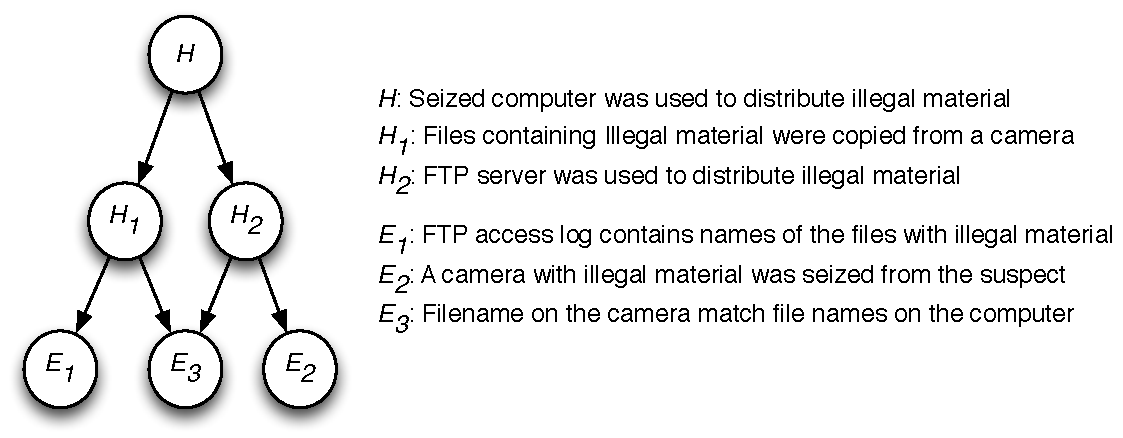
\includegraphics[width=\textwidth]{fig-1.pdf}
\caption{Bayesian belief network example}
\label{fig:bayesnet}
\end{figure}
 

Each node represents a proposition which is either true ($E_1$) or false ($\overline{E_1}$) The root nodes correspond to one or more overall investigative hypotheses, leaf nodes correspond to evidence items, and the interim nodes represent sub-hypotheses. Arrows in the tree represent causal dependency from parent to child nodes, and each arrow is associated with four conditional probabilities linking true and false values of the parent node with true and false values of the child node: For example, the arrow 
\includegraphics{insert.pdf} is associated with probabilities $P(E_1 \mid H_1)$,$P(\overline{E_1} \mid H_1)$,$P(E_1 \mid \overline{H_1})$,$P(\overline{E_1} \mid \overline{H_1})$. 

Given the prior probabilities of all nodes in the tree; conditional probabilities linking parent nodes to child nodes; and the actual values of some of the evidential assertions obtained through forensic examination, the posterior probability of the investigative hypotheses can be straightforwardly determined by recursive application of the Bayes rule from child nodes to the parent nodes.

\subsubsection{Prioritisation in probabilistic setting}

The problem of prioritisation in forensics can be expressed as a classical decision theoretic problem. Given the set $A$ of possible forensic tests that can be performed: $A=\left\{A_1,A_2,\dots,A_n\right\}$, the set of all possible outcomes for each test $O(A_i)=\left\{o_{i,1},o_{i,2},\dots o_{i,m} \right\}$, the utility function specifying desirability of each outcome $ u \colon O(A_i) \rightarrow \mathbb{R} $, and the likelihood of each outcome for each test: $P(o_{i,j} \mid A_i)$, it can be shown that if the cost of individual tests is negligible, the rational forensic scientist should choose the test that maximised expected utility across all possible outcomes:

\begin{equation}
\argmax_{i}\sum_{i=1}^{n}\sum_{j=0}^m P(o_{i,j}\mid A_i )u(o_{i,j} )
\end{equation}

Taroni and colleagues \cite{taroni2010data} explored prioritisation problem in the above setting with two mutually exclusive investigative hypotheses ($H_0$ and $H_1$) and a fixed number of forensic tests that could be carried out in any order.  They defined the utility of each test outcome to be proportional to the degree it makes one hypotheses more probable than the other:

\begin{equation}
u(o_{i,j} ) \propto \frac{P(H_0 \mid o_{i,j})}{P(H_1 \mid o_{i,j})}
\end{equation}

Overill and colleagues \cite{overill2009cost} adopted a different, and likely suboptimal approach. Their way of prioritising evidence examination is a two-stage process. In the first stage, relative weight $W_i$ and examination cost $T_i$ are assigned to each evidential object $O_i$  to be examined. In the second stage, the forensic examination is carried out in a greedy fashion: every time picking the object with the lowest relative cost, but the highest relative weight among all objects with that cost. 

Despite the ability to represent and reason with uncertain information, Bayesian belief networks have two main disadvantages:

\begin{itemize}

\item{The need to determine prior probabilities for the random variables represented in the model and the conditional probabilities linking events in computer system to evidence they produce.  Works of Kwan and Overill suggest obtaining them either from human experts, from statistical analysis of the evidential, or by using uninformed priors. The first two options are highly laborious, while the last option leads to imprecision.}

\item{The other big disadvantage is that the Bayesian belief networks are essentially propositional.  Not only it is difficult to establish prior probabilities, but if the configuration of the system under investigation is substantially different from the one used to build the network, it is not straightforward to adapt the existing model to the new circumstance.}

\end{itemize}

The sum-total of these disadvantages is that the probabilistic methods highlighted in this section are not being widely used in digital forensic practice. 


\section{Decision-theoretic File Carving}

\subsection{Approach}

\subsection{Formalization}

\section{Evaluation}

\subsection{Experimentation Design}

\subsection{Evaluation}

\subsubsection{Pro/Con}

\section{Conclusions}

\subsection{Future Work}

\bibliographystyle{ieeetr}
\bibliography{DECA}
	
\end{document}